\documentclass{article}
\usepackage{LectureNotes}

\setstretch{1.2}

\begin{comment}
\geometry{
    textheight=9in,
    textwidth=5.5in,
    top=1in,
    headheight=12pt,
    headsep=25pt,
    footskip=30pt
}
\end{comment}


\geometry
{
    a4paper,
    total={170mm,257mm},
    left=20mm,
    top=20mm,
}


% ------------------------------------------------------------------------------

\begin{document}

% ------------------------------------------------------------------------------
% Cover Page and ToC
% ------------------------------------------------------------------------------

\title{ \normalsize \textsc{}
		\\ [2.0cm]
		\HRule{1.5pt} \\
		\LARGE \textbf{\uppercase{40.002 Optimization}
		\HRule{2.0pt} \\ [0.6cm] \LARGE{An Introduction to Optimization} \vspace*{10\baselineskip}}
		}
\date{\today}
\author{\textbf{Michael Hoon}}

\maketitle
\newpage

\tableofcontents
\newpage

% ------------------------------------------------------------------------------

\section{Introduction to Linear Programming}
An optimization problem is defined by:

\begin{itemize}
    \item \textbf{Decision variables}: elements under the control of the decision maker
    \item \textbf{A (single) objective function}: a function of the decision variables that we want to optimize, corresponding to a criterion for measuring maximize
    \item \textbf{Constraints}: restrictions that define which values of the decision variables are allowed.
\end{itemize}

\noindent We want to find the \textbf{minimum} or \textbf{maximum} of a function of one or many variables subject to a set of \textbf{constraints}:

\begin{align}
    & \min \; f(x_{1}, \dots x_n) \\ \nonumber
    & \ni(x_{1}, \dots x_n) \in \chi \subseteq \mathbb{R}^{n}
\end{align}

\noindent where the decision variables are vectors $x_{1}, \dots x_n$, the objective function is $f(x_{1}, \dots x_n)$ and the constraints are defined by the set $\chi \subseteq \mathbb{R}^{n}$. A vector $\mathbf{x}^{*}$ is called \textit{optimal}, or a \textit{solution} of the problem, if it has the \textbf{smallest objective value} among all vectors that satisfy the constraints. 

\subsection{Standard Form}
A linear program is a class of optimisation problem in which the objective and all constraint functions are \textbf{linear}. For a minimisation problem,

\begin{align}
    & \min \; \mathbf{c}^{\top} \mathbf{x} \\ \nonumber
    & \ni \mathbf{Ax} \geq \mathbf{b}, \; \text{and} \; \mathbf{x} \geq 0
\end{align}

\noindent and for maximisation problems,

\begin{align}
    & \max \; \mathbf{c}^{\top} \mathbf{x} \\ \nonumber
    & \ni \mathbf{Ax} \leq \mathbf{b}, \; \text{and} \; \mathbf{x} \geq 0
\end{align}

\noindent where the decision vector is $\mathbf{x}$ (n variables), linear objective function: $f(\mathbf{x}) = \mathbf{c}^{\top} \mathbf{x} = \sum_{i=1}^{n} c_i x_i $, and the linear constraints are $\chi = \{\mathbf{x} \in \mathbb{R}^{n}\mid \mathbf{Ax} \geq \mathbf{b}\}$ (m constraints) \footnote{Note: vector inequalities are interpreted componentwise.}. Note that matrix $\mathbf{A}_{(m\times n)}$ is of $m \times n$ dimension. 

\subsubsection{Inequality Transformations}

We have matrix $\mathbf{A}$ given by:

\begin{equation*}
    \mathbf{A} = \begin{pmatrix}
        - & \mathbf{a_1}^{\top} & - \\ 
        \vdots & \vdots & \vdots \\ 
        - & \mathbf{a_m}^{\top} & -
    \end{pmatrix}
\end{equation*}

\begin{itemize}
    \item An equality constraint $\mathbf{a_i}^{\top} \mathbf{x} = b_i$ is equivalent to two equality constraints $\mathbf{a_i}^{\top} \mathbf{x} \leq b_i$ and $\mathbf{a_i}^{\top} \mathbf{x} \geq b_i$
    \item An inequality constraint $\mathbf{a_i}^{\top} \mathbf{x} \leq b_i$ is equivalent to the inequality constraint $-\mathbf{a_i}^{\top} \mathbf{x} \geq -b_i$ (Note the negatives applied to both sides of the inequality).
    \item Constraints such as $x_j \geq 0, \; x_j \leq 0$ can be expressed in the form $\mathbf{a_i}^{\top} \mathbf{x} \geq b_i$ by appropriately choosing $\mathbf{a}_i, \; b_i$.
\end{itemize}

\noindent Note that there is no simple analytic formula for the solution of a linear program, but there are a variety of effective methods for solving them, including Dantzig's simplex method, and the more recent interior-point methods. We cannot give the exact number of arithmetic operations required to solve a linear program, but we can establish rigorous bounds on the number of operations required to solve a linear program using an interior-point method (in practice, this is of the order $n^{2}m$, assuming $m \geq n$). 

\subsubsection{Terminology}

\begin{definition}
    We now introduce some terminology for geometric linear programming:
    \begin{itemize}
        \item A \textbf{linear function} $f : \mathbb{R}^{n} \to \mathbb{R}$ is a function of the form: \begin{equation*}
            f(x_{1}, \dots , x_n) = \sum_{i=1}^{n} a_i x_i, \quad a_i \in \mathbb{R}
        \end{equation*}
        \item A \textbf{hyperplane} in $\mathbb{R}^{n}$ is the set of points satisfying a single linear \textbf{equation}:
        \begin{equation*}
            a_{1}x_{1} + \dots + a_n x_n = b, \quad a_n \in \mathbb{R}
        \end{equation*}
        \item A \textbf{halfspace} in $\mathbb{R}^{n}$ is the set of points satisfying a single linear \textbf{constraint}: 
        \begin{equation*}
            a_{1}x_{1} + \dots + a_n x_n \geq b, \quad a_n, b \in \mathbb{R}
        \end{equation*}
        \noindent A halfspace is a \textbf{convex set}.
        \item An LP is \textbf{bounded} if there is some value $Z$ such that $\mathbf{c}^{\top}\mathbf{x} \leq Z$. 
        \item A \textbf{polyhedron} is a set that can be described by a finite number of halfspaces. A \textbf{polytope} is a \textbf{bounded} polyhedron. The polytope of an LP is \textbf{convex}, since it is the intersection of halfspaces (which are convex).
        \item An assignment of values to the decision variables is a \textbf{feasible solution} if it \textbf{satisfies all the constraints} (infeasible otherwise). The set of all feasible solutions is the \textbf{feasible region.}
        \item An \textbf{optimal solution} is a feasible solution that achieves the \textbf{best possible objective function value}. For a minimisation problem, $x^{*}$ is optimal \textbf{iff} $\mathbf{c}^{\top} \mathbf{x^{\top}} \leq \mathbf{c}^{\top} \mathbf{x}$ for all feasible $\mathbf{x}$. 
        \item We call $\mathbf{c}^{\top} x^{*}$ the \textbf{optimal objective value}. 
        \item $\forall K \in \mathbb{R}$ we can find a feasible solution $\mathbf{x}$ such that $\mathbf{c}^{\top}\mathbf{x} \leq K$, then the linear program in \textbf{minimisation} form has \textbf{unbounded} cost. The optimum cost is then $-\infty$. In this case, we can find a feasible $\mathbf{x}$ and direction $\mathbf{d}$ such that $\mathbf{x} + t \mathbf{d}$ is feasible $\forall t \geq 0$ and $\mathbf{c}^{\top}d < 0$.
    \end{itemize}    
\end{definition}

\noindent For every linear program, we know that one of the following cases must hold:

\begin{enumerate}
    \item The LP is infeasible. There is no value of $x$ that satisfies the constraints. 
    \item The LP has an optimal solution
    \item The LP is unbounded. 
\end{enumerate}

\noindent Mathematically, this follows from the fact that if the LP is \textbf{feasible and bounded}, then it is a closed and bounded subset of $\mathbb{R}^{n}$ and hence has a maximum point. 

\subsection{Geometric Definition}

In a simple two-dimensional space with the equation $x_{1} + x_{2} = z$, this function can be represented by a line. The decision variables are $x_{1}$ ad $x_{2}$, and this line represents all possible combinations of $x_{1}$ and $x_{2}$ that yield the same objective value $z$. \\ 

\noindent Each constraint is a linear inequality, which creates a boundary in the solution space. The feasible region is now the polygon formed by the intersection of all these constraint boundaries. \\

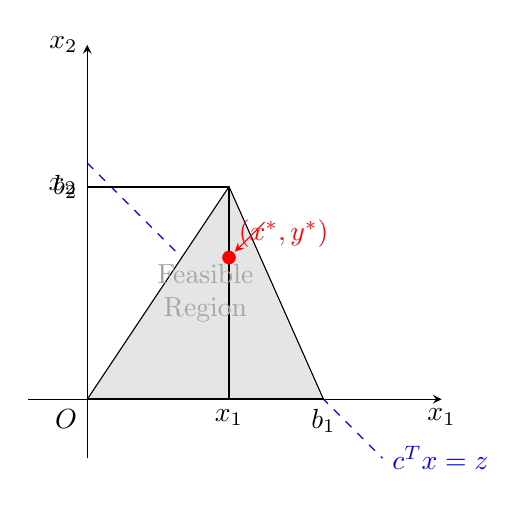
\begin{tikzpicture}[>=stealth, scale=1.5]
    % Objective function
    \draw[->] (-0.5,0) -- (3,0) node[below]{$x_1$};
    \draw[->] (0,-0.5) -- (0,3) node[left]{$x_2$};
    \draw[dashed, domain=0:2.5, variable=\x, blue] plot ({\x}, {2-\x}) node[right]{$c^Tx = z$};
  
    % Constraints
    \filldraw[fill=gray!20] (0,0) -- (2,0) -- (1.2,1.8) -- cycle;
    \draw[thick] (2,0) -- (0,0) node[below left]{$O$};
    \draw[thick] (1.2,1.8) -- (1.2,0) node[below]{$x_1$};
    \draw[thick] (1.2,1.8) -- (0,1.8) node[left]{$x_2$};
    
    % Labels
    \node[below] at (2,0) {$b_1$};
    \node[left] at (0,1.8) {$b_2$};
  
    % Optimal solution
    \filldraw[red] (1.2,1.2) circle (1.5pt) node[above right]{$(x^*,y^*)$};
    
    % Arrow to optimal solution
    \draw[->, red] (1.5,1.5) -- (1.25,1.25);
  
    % Feasible Region label
    \node[gray!70, align=center] at (1,0.9) {Feasible\\Region};
  \end{tikzpicture}

\noindent The feasible region is often convex, meaning that if points A and B are inside the region, the line segment connecting A and B are also inside the region. Some examples are shown below: \\

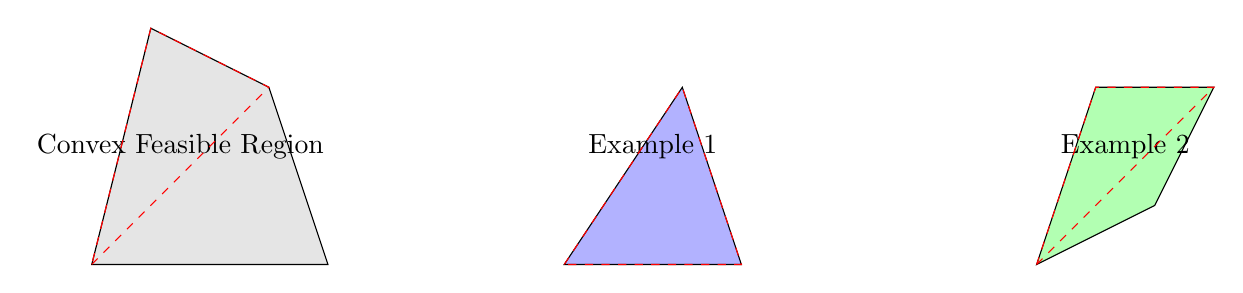
\begin{tikzpicture}[>=stealth, scale=1.5]
    % Convex Feasible Region
    \filldraw[fill=gray!20] (0,0) -- (2,0) -- (1.5,1.5) -- (0.5,2) -- cycle;
  
    % Convex Examples
    \filldraw[fill=blue!30, xshift=4cm] (0,0) -- (1.5,0) -- (1,1.5) -- cycle;
    \filldraw[fill=green!30, xshift=8cm] (0,0) -- (1,0.5) -- (1.5,1.5) -- (0.5,1.5) -- cycle;
  
    % Labels
    \node at (0.75,1) {Convex Feasible Region};
    \node at (4.75,1) {Example 1};
    \node at (8.75,1) {Example 2};
  
    % Convex Hulls
    \draw[dashed, red] (0,0) -- (1.5,1.5) -- (0.5,2) -- (0,0);
    \draw[dashed, red, xshift=4cm] (0,0) -- (1,1.5) -- (1.5,0) -- (0,0);
    \draw[dashed, red, xshift=8cm] (0,0) -- (1.5,1.5) -- (0.5,1.5) -- (0,0);
  \end{tikzpicture} \\


\subsection{Graphical Approach}

Solving the LP via a graphical approach involves drawing the halfspaces defined by the constraints, as well as the iso-lines defined by the optimisation problem. \\

\begin{figure}[H]
    \centering
    \includegraphics[width=0.5\textwidth]{Images/LP_Graphical.png}
    \caption{A linear Program in 2 dimensions}
    \label{fig:lpdiag}
\end{figure} 

\noindent After determining the bounded-ness of the LP problem, shade the feasible region (polytope) defined by the constraints. Points within this feasible region satisfy all constraints, and is a \textbf{convex polygon}. \\

\noindent Note that the feasible region for an LP may be \textit{empty, a single point, or infinite (unbounded)}. Our goal now is to find a point in the feasible region that optimises this objective. Since there are an infinite number of possible points within the polytope, we need to reduce this space. 

\begin{theorem}
    The maximum point for an LP is always achieved at one of the vertices of a polytope. In general, if there are $n$ dimensions (variables), a vertex may occur wherever $n$ (linearly independent) hyperplanes (i.e. constraints) intersect.
\end{theorem}

\noindent Recall in linear algebra that if you have $n$ linearly independent equations and $n$ variables, there is only one optimal solution (and if they are not linearly independent - you have infinitely many solutions). So in a system with $m$ constraints and $n$ variables, there are $\binom{m}{n} = O(m^{n})$ vertices. \\ 

\noindent Now, to determine which of the vertices gives the maximum objective value, we can substitute the variables into the objective function and compare the final values \footnote{Note that at each vertex, if the iso-line falls within the polytope, then it is not a maximum.} 

\subsubsection{Geometric Intuition}
The objective function gives the optimisation direction, and the goal is to find the feasible point that is furthest in this direction. 

\subsection{Convexity}
When optimisation is concerned, we equate "convex" with "nice", and "non-convex" with "nasty". 

\subsubsection{Convex Sets}

\begin{theorem}
    The feasible region (Polytope) of an LP is \textbf{convex}. 
\end{theorem}

\noindent Intuitively, a subset $C\subseteq \mathbb{R}^{n}$ is convex if it is "filled in", meaning that it contains all line segments between its points (if you draw a line segment between two points of the region, the line segment itself must be in the region). 

\begin{figure}[H]
    \centering
    \includegraphics[width=0.7\textwidth]{Images/convexity.png}
    \caption{Examples of convex and non-convex sets}
    \label{fig:1-convex}
\end{figure} 

\noindent Mathematically, a set $\chi \subseteq \mathbb{R}^{n}$ is convex if 

\begin{equation*}
    \lambda \mathbf{x} + (1-\lambda)\mathbf{y} \in \chi, \; \forall \mathbf{x}, \mathbf{y} \in \chi, \; \forall \lambda \in [0,1]
\end{equation*}

As $\lambda$ ranges from 0 to 1, it traces out the line segment from $\mathbf{y}$ to $\mathbf{x}$.

\subsubsection{Convex Functions}
We define a function $f:\mathbb{R}^{n} \to \mathbb{R}$ to be \textit{convex} if and only if the region above its graph is a convex set. 
\begin{figure}[H]
    \centering
    \includegraphics[width=0.7\textwidth]{Images/convexityfn.png}
    \caption{Examples of convex and non-convex functions}
    \label{fig:1-convexfns}
\end{figure} 

\noindent Equivalently, a convex function is one where all "chords" of its graph lie above the graph. Mathematically,

\begin{equation}
    f(\lambda \mathbf{x} + (1-\lambda)\mathbf{y}) \leq \lambda f(\mathbf{x}) + (1-\lambda) f(\mathbf{y}), \; \forall \; \mathbf{x}, \mathbf{y} \in \mathbb{R}^{n}, \; \forall \lambda \in [0,1]
\end{equation}

\begin{figure}[H]
    \centering
    \includegraphics[width=0.6\textwidth]{Images/convexityfn2.png}
    \caption{Visualisation of a convex function}
    \label{fig:1-convexfns2}
\end{figure} 

\noindent That is, for points $\mathbf{x}$ and $\mathbf{y}$, if you take the average of $\mathbf{x}$ and $\mathbf{y}$, and then apply $f$, you'll get a smaller number than if you first apply $f$ to $\mathbf{x}$ and $\mathbf{y}$, and then average the results. Likewise, a function $f$ is \textbf{concave} if $-f$ is convex.

\subsubsection{Why Convexity Helps}
Consider the case where the feasible region or the objective function is not convex. With a non-convex feasible region, there can be "locally optimal" feasible points that are not globally optimal, even with a linear objective function. The same problem arises with a non-convex objective function, even when the feasible region is just the real line. When both the objective function and feasible region are convex, this cannot happen - \textbf{all local optima are also global optima} (which makes optimisation easier).

\begin{theorem}
    Let $\chi$ be a convex set and $f(x)$ be a convex function. Then:
    \begin{align*}
        \min & \; f(x) \\ 
        \text{s.t.} & \; \; x \in \chi \subseteq \mathbb{R}^{n}
    \end{align*}
    \noindent is a convex optimisation problem. A key property of such a convex optimisation problem that is a \textbf{local minimum is always the global minimum}. 
\end{theorem}

\begin{figure}[H]
    \centering
    \includegraphics[width=0.8\textwidth]{Images/convexityfn3.png}
    \caption{Non-convexity and local optima. (Left) A linear (i.e. convex) objective function with a non-convex feasible region. (Right) A non-convex objective function over a convex feasible region (the real line).}
    \label{fig:1-convexfns3}
\end{figure} 

\subsubsection{First-Order Characterisation}
Suppose a function $f: \mathbb{R}^{n} \to \mathbb{R}$ is differentiable \footnote{the gradient $\nabla_x f(x)$ exists at all points $x$ in the domain of $f$. It is defined as $\nabla_x f(x) \in \mathbb{R}^{n}, \; (\nabla_x f(x))_i = \frac{\partial f(x)}{\partial x_i}$}. Then $f$ is convex if and only if $D(f)$ is a convex set and for all $x, y \in D(f)$:

\begin{equation}
    f(y) \geq f(x) + \nabla_x f(x)^{\top} (y-x)
\end{equation}

\noindent The function on the right is called the \textbf{first order approximation} to $f$ at the point $x$. 

\begin{theorem}
    The first order condition for convexity says that $f$ is convex if and only if the tangent line is a global underestimator of the function $f$. i.e. if we draw a tangent line at any point (refer to Figure \ref{fig:1-firstoderconvex}), then every point on this line will lie below the corresponding point on $f$. 
\end{theorem}

\begin{figure}[H]
    \centering
    \includegraphics[width=0.6\textwidth]{Images/firstoderconvexity.png}
    \caption{Illustration of first-order condition for convexity}
    \label{fig:1-firstorderconvex}
\end{figure} 


\subsubsection{Second-Order Characterisation}
Suppose that a function $f: \mathbb{R}^{n} \to \mathbb{R}$ is twice differentiable (i.e. the Hessian $\nabla^{n}_x f(x)$ is defined for all $x$ in the domain of $f$). Then $f$ is convex if and only if $D(f)$ is a convex set and its Hessian is positive semidefinite (PSD): i.e. for any $x \in D(f)$, 

\begin{equation}
    \nabla^{2}_x f(x) \succeq 0 
\end{equation}

\noindent where $\succeq$ denotes PSD-ness. In one-dimension, this is equivalent to the condition that the second derivative $f''(x)$ always be non-negative. \\ 

\noindent The Hessian is defined as:

\begin{equation}
    \nabla^{2}_x f(x) \in \mathbb{R}^{n \times n}, \quad (\nabla^{2}_x f(x))_{ij} = \frac{\partial^{2} f(x)}{\partial x_i \partial x_j}
\end{equation}


\begin{theorem}
    We can see that $f$ is \textbf{strictly convex} if its Hessian is \textbf{Positive Definite}, concave if it is \textbf{Negative Semidefinite}, and \textbf{strictly concave} if it is \textbf{Negative Definite}.
\end{theorem}


\subsubsection{Solving Convexity-Related Questions}

\subsection{Some Matrix Calculus}

\subsubsection{The Gradient}

\begin{definition}
    
Suppose that $f: \mathbb{R}^{m\times n}\to \mathbb{R}$ is a function that takes as input a matrix $A$ of size $m\times n$ and returns a real value. Then the \textbf{gradient} of $f$ (with respect to $A\in \mathbb{R}^{m\times n}$) is the matrix of \textbf{partial derivatives}:

\begin{equation}
    \nabla_A f(A) \in \mathbb{R}^{m\times n} = \begin{bmatrix}
        \frac{\partial f(A)}{\partial A_{11}} & \frac{\partial f(A)}{\partial A_{12}} & \dots & \frac{\partial f(A)}{\partial A_{1n}} \\ 
        \frac{\partial f(A)}{\partial A_{21}} & \frac{\partial f(A)}{\partial A_{22}} & \dots & \frac{\partial f(A)}{\partial A_{2n}} \\ 
        \vdots & \vdots & \ddots & \vdots \\ 
        \frac{\partial f(A)}{\partial A_{m1}} & \frac{\partial f(A)}{\partial A_{m2}} &  \dots & \frac{\partial f(A)}{\partial A_{mn}}
    \end{bmatrix}
\end{equation}

\end{definition}

\noindent Note that the gradient of a function \footnote{Gradients are a natural extension of partial derivatives to functions of multiple variables.} is only defined if the function is real-valued, i.e. if it returns a scalar value. \\

\noindent Some equivalent properties of the gradient from partial derivatives:

\begin{enumerate}
    \item $\nabla_x (f(x) + g(x)) = \nabla_x f(x) + \nabla_x g(x)$
    \item For $t \in \mathbb{R}, \; \nabla_x(t f(x)) = t\nabla_x f(x)$
\end{enumerate}

\subsubsection{The Hessian}

\begin{definition}
    
Suppose that $f: \mathbb{R}^{n}\to \mathbb{R}$ is a function that takes a vector in $\mathbb{R}^{n}$ and returns a real number. Then the \textbf{Hessian} with respect to $x$, written $\nabla^{2}_x f(x)$ is the $n\times n$ matrix of partial derivatives:


\begin{equation}
    \nabla^{2}_x f(x) \in \mathbb{R}^{n\times n} = \begin{bmatrix}
        \frac{\partial^{2} f(x)}{\partial x^{2}_{1}} & \frac{\partial^{2} f(x)}{\partial x_{1}\partial x_{2}} & \dots & \frac{\partial f(x)}{\partial x_{1} \partial x_n} \\ 
        \frac{\partial f(x)}{\partial x_{2} \partial x_{1}} & \frac{\partial f(x)}{\partial x^{2}_{2}} & \dots & \frac{\partial f(x)}{\partial x_{2} \partial x_n} \\ 
        \vdots & \vdots & \ddots & \vdots \\ 
        \frac{\partial f(x)}{\partial x_{n} \partial x_{1}} & \frac{\partial f(x)}{\partial x_{n} \partial x_{2}} &  \dots & \frac{\partial f(x)}{\partial x^{2}_{n}}
    \end{bmatrix}
\end{equation}

\end{definition}

\noindent Note that the Hessian is always symmetric, since 

\begin{equation*}
    \frac{\partial^{2} f(x)}{\partial x_i \partial x_j} = \frac{\partial^{2}}{\partial x_j \partial x_i}
\end{equation*}

\noindent The Hessian is defined only when $f(x)$ is real-valued. Note that for functions of a vector, the gradient of the function is a vector, and we cannot take the gradient of a vector.\textbf{ Therefore, it is not the case that the Hessian is the Gradient of the Gradient}. 

\subsubsection{Definite Matrix \& Eigenvalues}

\begin{definition}

    Let $M$ be an $n \times n$ Hermitian Matrix \footnote{A complex square matrix that is equal to its own conjugate transpose: $A = \overline{A^{\top}}.$}(including Symmetric Matrices \footnote{A square matrix that is equal to its transpose.}). All eigenvalues of $M$ are real, and their sign characterise its definite-ness:

    \begin{enumerate}
        \item $M$ is \textbf{Positive Definite} if and only if all of its eigenvalues are \textbf{positive}.
        \item $M$ is \textbf{Positive Semi-Definite} if and only if all its eigenvalues are \textbf{non-negative}. 
        \item $M$ is \textbf{Negative Definite} if and only if all of its eigenvalue are \textbf{negative}.
        \item $M$ is \textbf{Negative Semi-Definite} if and only if all if its eigenvalues are \textbf{non-positive}. 
        \item $M$ is \textbf{indefinite} if and only if it has both positive and negative eigenvalues.
    \end{enumerate}

\end{definition}


\section{Simplex Method}

\subsection{The True Standard Form}
Previously, we know that a linear program can take either a maximisation of minimisation form, depending on the context. The constraints thus can either be inequalities or equalities. Some variables might be unrestricted in sign, while others might be restricted to be non-negative. \\ 

\noindent A linear program is said to be in \textit{standard form} if the following hold: 

\begin{enumerate}
    \item It is a minimisation program.
    \item There are only equalities (no inequalities) and 
    \item All variables are restricted to be non-negative. 
\end{enumerate}

\noindent In matrix form, we have 

\begin{align}\label{eq:2-standard form}
    \min \quad & c^{\top}\mathbf{x} \\ \nonumber 
    \text{s.t.} \quad & \mathbf{Ax} = \mathbf{b} \\ \nonumber 
    \quad & \mathbf{x} \geq 0 
\end{align}

\noindent where $n$ is the number of decision variables and $m$ is the number of equality constraints and $\mathbf{0}$ is a vector of zeros. 

\subsubsection{Transformation Tricks}
We have a few transformation tricks to convert any LP into the true standard form:

\begin{enumerate}
    \item Eliminate non-positive and free variables (unrestricted in sign): \begin{align*}
        & x_j \leq 0 \to \text{Let} \; \hat{x}_j = -x_j \; \text{and set } \hat{x}_j \geq 0 \\ 
        & x_j \text{is free } \to \text{Let } x_j = x_j^+ - x_j^- \text{ and set } x_j^+, x_j^- \geq 0  
    \end{align*}
    \item If we have an inequality constraint $a_{i1}x_{1}+ \dots + a_{in}x_n \leq b$, then we can transform it into an equality constraint by adding a \textit{slack} variable $s_i$, restricted to be non-negative: \begin{equation*}
        a_{i_{1}} x_{1} + \dots + a_{in}x_n + s_i = b_i, \quad s_i \geq 0
    \end{equation*}
    \item Similarly, if we have an inequality constraint $a_{i_{1}}x_{1} + \dots + a_{in} x_n \geq b_i$ then we can transform it into an equality constraint by adding a \textit{surplus} variable, $s_i$, restricted to be non-negative: \begin{equation*}
        a_{i_{1}}x_{1} + \dots + a_{in}x_n - s_i = b_i, \quad s_i \geq 0 
    \end{equation*}
\end{enumerate}

\subsection{Active Constraints}

\begin{enumerate}
    \item A constraint is said to be \textbf{active} at a point $\mathbf{x}$ if the constraint is satisfied at equality at that point. 
    \item A set of linear constraints are linearly independent if their coefficient vectors are linearly independent; else they are linearly dependent. 
\end{enumerate}

\subsection{Optimality Test of LP in Inequality Form}

\begin{figure}[H]
    \centering
    \includegraphics[width=0.6\textwidth]{Images/LPGeometry.png}
    \caption{Feasible Region with Objective Contours}
    \label{fig:2-lpgeometry}
\end{figure} 

Consider an LP with $m$ variables and $n$ linear inequality constraints. \begin{enumerate}
    \item A \textbf{Corner Point} is an intersection point of the hyperplanes of $m$ linearly-independent inequality constraints. 
    \item These constraints are called active constraints at the corner solution.
    \item Two corner solutions are adjacent if they differ by one active constraint.
\end{enumerate}

\begin{theorem}
    For an LP in the standard form, a \textbf{Corner Point} is maximal if and only if the objective vector is a conic combination of the normal direction vectors of the $m$ hyperplanes. Refer to Figure \ref{fig:2-lpgeometry}. 
\end{theorem}


\subsection{Some Polyhedron Definitions}

Let $P \subseteq \mathbb{R}^{n}$ be a non-empty polyhedron. 

\begin{enumerate}
    \item A vector $\mathbb{x} \in P$ is an \textbf{extreme point} of $P$ if we cannot find two vectors $\mathbf{y}, \mathbf{z} \in P$, both different from $\mathbf{x}$, and a scalar $\lambda \in [0,1]$, such that $\mathbf{x} = \lambda \mathbf{y} + (1- \lambda) \mathbf{z} $ (Geometric Definition). 
    \item A vector $\mathbf{x} \in P$ is a \textbf{vertex} of $P$ if there exists some $\mathbf{c}$ such that $\mathbf{x}$ is the unique minimizer of the LP $\min \{\mathbf{c}^{\top}\mathbf{y} \mid \mathbf{y} \in P\}$ (Optimisation definition)
    \item A vector $\mathbf{x} \in P$ is a \textbf{basic feasible solution} (BFS) if there exists $n$ linearly independent constraints that are active at $\mathbf{x}$ (including both inequality and equality constraints) (Algebraic definition). 
\end{enumerate}

\begin{theorem}
    Let $P \subseteq \mathbb{R}^{n}$ be a nonempty polyhedron and let $x^{*} \in P$. Then: \begin{equation*}
        x^{*} \text{ is an extreme point } \Longleftrightarrow x^{*} \text{ is a vertex } \Longleftrightarrow x^{*} \text{ is a BFS.}
    \end{equation*} Notably, these 3 are the same definitions but in different form.
\end{theorem}


\subsection{Finding a Basic Feasible Solution}
We can "eyeball" a BFS by the following steps: \\ 

\noindent Consider an LP where: 

\begin{enumerate}
    \item LP is of standard form
    \item The right hand side vector $\mathbf{b}$ is non-negative
    \item The constraint matrix contains the identity matrix $I$ as a \textbf{submatrix} (or a permutation of the identity matrix). 
\end{enumerate}

\noindent Then, we can easily identify a BFS:

\begin{enumerate}
    \item Variables associated with $I$ (or permutations of $I$) are \textbf{basic variables}. THey take the value of the right hand side vector. Other variables are nonbasic variables; they take values of zero. 
    \item Columns of the constraint matrix corresponding to the basic variables form a \textbf{basis}; we also refer to the set of basic variables sometimes as a basis. 
\end{enumerate}

\subsection{The Simplex Method}
To use the Simplex Method on an LP, we shall assume the following:

\begin{enumerate}
    \item The LP is in standard form
    \item $b \geq 0$
    \item There exists a collection $B$ of $m$ variables called a \textit{basis} such that: \begin{enumerate}
        \item the submatrix $A_B$ of $A$ consisting of the columns of $A$ corresponding to the variables in $B$ is the $m \times m$ identity matrix
        \item the cost coefficients corresponding to the variables in $B$ are all equal to 0. 
    \end{enumerate}
\end{enumerate}


\subsection{Slack Variables and Pivoting}

Simplex method is an iterative procedure which corresponds, geometrically, to moving from one feasible corner to another until optimal feasible point is located. Slack variables are introduced to ensure corner points are \textit{feasible}, not outside solution region. Algebraically, hopping from one feasible corner point to another corresponds to repeatedly identifying \textit{pivot column}, \textit{pivot row}, and consequently, \textit{pivot element}, in a succession of matrix tableaus. Having identified pivot element, a new tableau is created by \textit{pivoting} (Gauss-Jordan method) on this element. 

\subsection{Algorithmic Approach}\label{sec:2-algorithmicapproach}
The steps of the simplex algorithm can be carried out using a simplex tableau. We have the LP in standard form: \begin{align*}
    \min \quad & -3 x_{1} -2 x_{2} \\ 
    \text{s.t.} \quad & x_{1} -x_{2} + x_{3} = 1 \\ 
    & 2 x_{1} + x_{2} \qquad + x_{4} = 4 \\ 
    & \qquad x_{2} \qquad \quad \qquad + x_{5} = 2 \\ 
    & x_{1}, x_{2}, x_{3}, x_{4}, x_{5} \geq 0 
\end{align*}

\begin{table}[H]
    \centering
    \begin{tabular}{c | c c | c c c c c}
        Row & & & $x_{1}$ & $x_{2}$ & $x_{3}$ & $x_{4}$ & $x_{5}$ \\ \hline 
        $R_{0}$ & & 0 & -3 & -2 & 1 & 0 & 0 \\ \hline 
        $R_{1}$ & $x_{3}$ & 1 & 1 & -1 & 0 & 0 & 0 \\ 
        $R_{2}$ & $x_{4}$ & 4 & 2 & 1 & 0 & 1 & 0 \\ 
        $R_{3}$ & $x_{5}$ & 2 & 0 & 1 & 0 & 0 & 1
    \end{tabular}
    \caption{Simple Tableau}
    \label{tab: 2-tableau}
\end{table} 

\noindent In this example, $B = \{x_{4}, x_{5}, x_{6}\}$. The variables in $B$ are called basic variables while the others are \textit{nonbasic}. The set of nonbasic variables is denoted by $N = \{x_{1}, x_{2}, x_{3}\}$. We now have a matrix $A_B = I$, where it is easier to quickly infer the values of the basic variables given the values of the nonbasic variables\footnote{Only if the constraint matrix contains the identity matrix as a submatrix (or a permutation of it). Then, the basic variables take the value of the right hand side vector, while the others (nonbasic) are zero.}. \\ 


\subsubsection{Basic Feasible Solutions (BFS)} 
Furthermore, we don't need to know the values of the basic variables to evaluate the cost of the solution (there is no guarantee however that the solution is feasible). By setting all nonbasic variables to be 0, the values of the basic variables are just given by the right-hand-sides of the constraints. The simplex method is an iterative method that generates a sequence of BFS (corresponding to different bases) and eventually stops when it has found an optimal basic feasible solution. \\ 

\noindent At this point, to move to a better solution, we can use the ratio test: 

\begin{theorem}
    \textbf{Minimum Ratio Test}: When introducing variable $x_s$ into the basis, identify the row that gives the \textbf{minimum ratio of left-hand side values} in the tableau to the corresponding $x_s$ coefficient in the chosen column. Compute these ratios only for constraints that have positive coefficients for $x_s$. 
\end{theorem}

\noindent In this case, we have \begin{equation*}
    t^{*} = \min \left(\frac{1}{1}, \frac{4}{2}\right) = 1
\end{equation*}

\noindent In particular, $x_{1}$ enters the basis and $x_{3}$ leaves the basis. Do row operations using this identified row (leaving variable) such that for the chosen column, (entering variable), we \textbf{obtain a 1 in the entry where they intersect and 0 otherwise}. Now, after pivoting $(R_{0} \to R_{0}  + 3 R_{1}, \; R_{2} \to  R_{2} - 2 R_{1})$:


\begin{table}[H]
    \centering
    \begin{tabular}{c | c c | c c c c c}
        Row & & & $x_{1}$ & $x_{2}$ & $x_{3}$ & $x_{4}$ & $x_{5}$ \\ \hline 
        $R_{0}$ & & 3 & 0 & -5 & 3 & 0 & 0 \\ \hline 
        $R_{1}$ & $x_{1}$ & 1 & 1 & -1 & 0 & 0 & 0 \\ 
        $R_{2}$ & $x_{4}$ & 2 & 0 & 3 & -2 & 1 & 0 \\ 
        $R_{3}$ & $x_{5}$ & 2 & 0 & 1 & 0 & 0 & 1
    \end{tabular}
    \caption{Next Pivot}
    \label{tab: 2-tableaupivoted2}
\end{table} 

\noindent At this point, we now see: \begin{enumerate}
    \item BFS is $(x_{1}, x_{2}, x_{3}, x_{4}, x_{5}) = (1,0,0,2,2)$, identified by the variables on the left of the tableau $(x_{1}, x_{4}, x_{5})$. 
    \item Objective function value is $-3$ (negative of value of top left entry). 
    \item However, $x_{2}$ has negative cost in the top row, so the solution is still non-optimal.
    \item Note that the element that we are pivoting on must always end up being 1.
\end{enumerate}

\noindent We now apply the minimum ratio test again: \begin{equation*}
    t^{*} = \min \left(\frac{2}{3}, \frac{2}{1}\right) = \frac{2}{3}
\end{equation*}

\noindent where $x_{4}$ leaves, and $x_{2}$ enters. We now perform the row operations $(R_{2} \to \frac{R_{2}}{3}, \; R_{0} \to  R_{0} + 5 R_{2}, \; R_{1} \to  R_{1} + R_{2}, \; R_{3} \to R_{3}-R_{2})$. We obtain the next tableau:


\begin{table}[H]
    \centering
    \begin{tabular}{c | c c | c c c c c}
        Row & & & $x_{1}$ & $x_{2}$ & $x_{3}$ & $x_{4}$ & $x_{5}$ \\ \hline 
        $R_{0}$ & & 19/3 & 0 & 0 & -1/3 & 5/3 & 0 \\ \hline 
        $R_{1}$ & $x_{1}$ & 5/3  & 1 & 0 & 1/3 & 1/3 & 0 \\ 
        $R_{2}$ & $x_{4}$ & 2/3 & 0 & 1 & -2/3 & 1/3 & 0 \\ 
        $R_{3}$ & $x_{5}$ & 4/3 & 0 & 0 & 2/3 & -1/3 & 1
    \end{tabular}
    \caption{Simplex Tableau after pivoting again}
    \label{tab: 2-tableaupivoted3}
\end{table} 

\noindent Applying the minimum ratio test again, \begin{equation*}
    t^{*} = \min \left( \frac{5/3}{1/3}, \frac{4/3}{2/3}\right) = 2
\end{equation*}

\noindent Since we still have negative cost in $x_{3}$, $x_{5}$ leaves the basis, while $x_{3}$ enters. We perform the row operations: $(R_{0} \to R_{0} + \frac{R_{3}}{2}, \; R_{1} \to R_{1}-\frac{R_{3}}{2}, \; R_{2} \to R_{2}+R_{3}, \; R_{3} \to \frac{R_{3}}{2/3})$.


\begin{table}[H]
    \centering
    \begin{tabular}{c | c c | c c c c c}
        Row & & & $x_{1}$ & $x_{2}$ & $x_{3}$ & $x_{4}$ & $x_{5}$ \\ \hline 
        $R_{0}$ & & 7 & 0 & 0 & 0 & 3/2 & 1/2 \\ \hline 
        $R_{1}$ & $x_{1}$ & 1  & 1 & 0 & 0 & 1/2 & -1/2 \\ 
        $R_{2}$ & $x_{4}$ & 2 & 0 & 1 & 0 & 0 & 1 \\ 
        $R_{3}$ & $x_{5}$ & 2 & 0 & 0 & 1 & -1/2 & 3/2 
    \end{tabular}
    \caption{Final Simplex Tableau }
    \label{tab: 2-finaltableau}
\end{table} 


\noindent At this point, all entries are nonnegative in $R_{0}$ for columns corresponding to $x_{1}$ to $x_{5}$. \textbf{The simplex algorithm terminates}. The optimal solution is now $x_{1} = 1, x_{2} = 2$, with optimal objective value being $z=-7$. 

\subsection{Simplex Method: Matrix Form}

Consider an LP in standard form, with $n$ variables and $m$ equality constraints, and the rows of $\mathbf{A}$ are linearly independent ($m \leq n$). Index the $m \times n$ matrix $ \mathbf{A}$ using column vectors: \begin{equation*}
    \mathbf{A} = \begin{pmatrix}
        | & & | \\ 
        \mathbf{A}_1 & \dots & \mathbf{A}_n \\ 
        | & & | 
    \end{pmatrix}
\end{equation*}

\noindent We start with a basis matrix $ \mathbf{B}$ where $B_{1}, \dots , B_m$ are the indices of the basic variables and $\mathbf{B} = (\mathbf{A}_{B_{1}}, \dots , \mathbf{A}_{B_m})$. $ \mathbf{B}$ is of size $m \times m $ and invertible, partitioning the matrix as $ \mathbf{A} = \begin{pmatrix}
    \mathbf{B} & \mathbf{N}
\end{pmatrix}$ (basic and nonbasic), the vector $\mathbf{x}$ to $\mathbf{x}_B$ and $\mathbf{x}_N$ and the cost vector $\mathbf{c}$ to $\mathbf{c}_B$ and $\mathbf{c}_N$ (the cost vector is the coefficients of the objective function). \\ 

\noindent To find an associated solution, we set $\mathbf{x}_N = \mathbf{0}$, and $\mathbf{x}_B = \mathbf{B}^{-1} \mathbf{b}$. If $\mathbf{B}^{-1} \mathbf{b} \geq 0$, this is a BFS. The objective value at the BFS is $z = \mathbf{c}^{\top}_B \mathbf{B}^{-1}\mathbf{b}$. See that we now have \begin{equation*}
    \mathbf{A} = \begin{pmatrix}
        \mathbf{B} & \mathbf{N}
    \end{pmatrix} 
\end{equation*}

\begin{equation*}
    \mathbf{x} = \begin{pmatrix}
        \mathbf{x}_B \\ 
        \mathbf{x}_N
    \end{pmatrix}^{m}_{n-m} \qquad \mathbf{c} = \begin{pmatrix}
        \mathbf{c}_B \\ 
        \mathbf{c}_N
    \end{pmatrix}
\end{equation*}

\subsubsection{Objective Value \& Solution}

By setting the variables $\mathbf{x}_N$ of $\mathbf{x}$ corresponding to the remaining columns of $\mathbf{A}$ equal to 0, we obtain a solution $\mathbf{x}$ of $\mathbf{A}\mathbf{x} = \mathbf{b}$: \begin{equation*}
    \begin{pmatrix}
        \mathbf{B} & \mathbf{N}
    \end{pmatrix} \begin{pmatrix}
        \mathbf{x}_B \\ 
        \mathbf{x}_N
    \end{pmatrix} = \mathbf{b} \Longleftrightarrow\mathbf{B}\mathbf{x}_B + \mathbf{N}\cancelto{0}{\mathbf{x}_N} = \mathbf{b}
\end{equation*}

\noindent We now have $\mathbf{x}_B = \mathbf{B}^{-1}\mathbf{b}$. \begin{theorem}
    When $\mathbf{x}_B = \mathbf{B}^{-1}\mathbf{b} \geq 0$, the solution is a BFS. The objective value at this BFS is: \begin{equation*}
        \mathbf{c}^{\top} \mathbf{x} = \begin{pmatrix}
            \mathbf{c}^{\top}_B & \mathbf{c}^{\top}_N
        \end{pmatrix} \begin{pmatrix}
            \mathbf{x}_B \\ 
            \mathbf{x}_N 
        \end{pmatrix} = \mathbf{b} \implies \mathbf{c}^{\top}_B \mathbf{x}_B + \mathbf{c}^{\top}_N \cancelto{0}{\mathbf{x}_N} = \mathbf{c}^{\top}_B \mathbf{B}^{-1}\mathbf{b}
    \end{equation*}
\end{theorem}

\noindent Suppose that we want to move from $\mathbf{x}$ to a new vector $\mathbf{x} + t \mathbf{d}$ by selecting a nonbasic variable $x_j$ (at zero level) and increasing it while keeping all other nonbasic variables at 0. The vector $\mathbf{d}$ is the direction vector. \\ 

\noindent We want to ensure that $\mathbf{x} + t \mathbf{d}$ is feasible for some $t > 0$. Thus, $\mathbf{A}(\mathbf{x} + t \mathbf{d}) = \mathbf{d} \implies \mathbf{Ad} = 0$. \begin{align*}
    \mathbf{Ad} = \mathbf{0} &\Longleftrightarrow \mathbf{B}\mathbf{d}_B + \mathbf{N}\mathbf{d}_N = \mathbf{0} \\ 
    & \Longleftrightarrow \mathbf{d}_B = - \mathbf{B}^{-1}\mathbf{N}\mathbf{d}_N
\end{align*}

\noindent When $\mathbf{d}_N$ has 1 for the $j$th entry and 0 otherwise, this gives us $\mathbf{d}_B = - \mathbf{B}^{-1}\mathbf{A}_j$, which is the direction vector for the basic variables. 

\subsubsection{Minimum Ratio Test}
We want to ensure that the direction value is in the \textbf{positive (largest) direction} (since we want to move to the optimum point). To set a bound on the value of $t$ in $\mathbf{x} + t \mathbf{d}\geq 0$: \begin{enumerate}
    \item If $\mathbf{d} \geq 0$, then $\mathbf{x} + t \mathbf{d} \geq 0 \; \forall t \geq 0$, and we can choose $t^{*} = \infty$ (objective is unbounded). 
    \item If $d_i <0$ for some $i$, then $x_i + td_i \geq \mathbf{0}$ gives $t \leq - \frac{x_1}{d_i}$  
\end{enumerate}

\begin{definition}
    We have the Minimum Ratio Test (MRT) \begin{equation*}
        t^{*} = \min_{\{i | d_i < 0\}} \left\{ -\frac{x_i}{d_i}\right\}
    \end{equation*} We only need to consider the basic variables while performing the ratio test, as for nonbasic variables we have $\mathbf{x}_N = \mathbf{0}$. 
\end{definition}

\subsubsection{Reduced Cost}

After moving in the specific direction of the largest change in cost, we want to calculate this rate of change in cost. This is given by: \begin{align*}
    \frac{\mathbf{c}^{\top}(\mathbf{x} + t \mathbf{d} - \mathbf{c}^{\top} \mathbf{x})}{t} &= \mathbf{c}^{\top}\mathbf{d} \\ 
    \implies \mathbf{c}^{\top} \mathbf{d} = \mathbf{c}^{\top}_B \mathbf{d}_B + c_j (1) &= c_j - \mathbf{c}^{\top}_B \mathbf{B}^{-1}\mathbf{A}_j
\end{align*}

\begin{definition}
    In LP, reduced cost (opportunity cost) is the amount by which an objective function coefficient would have to improve before it would be possible for a corresponding variable to assume a positive value in the optimal solution (for the variables to become non-basic and  enter the solution with a positive value). We define the reduced cost of each variable $x_j$ as: \begin{equation*}
        \bar{c}_j = c_j - \mathbf{c}^{\top}_B \mathbf{B}^{-1}\mathbf{A}_j
    \end{equation*}
    and the vector of reduced costs as: \begin{equation*}
        \mathbf{\bar{c}}^{\top} = \mathbf{c}^{\top} - \mathbf{c}^{\top}_B \mathbf{B}^{-1}\mathbf{A}
    \end{equation*}
\end{definition}

\noindent For $\mathbf{A} = \begin{pmatrix}
    \mathbf{B} & \mathbf{N}
\end{pmatrix}$, we can write $\mathbf{c} = \begin{pmatrix}
    \mathbf{c}_B & \mathbf{c}_N
\end{pmatrix}$, then we have \begin{equation*}
    \mathbf{\bar{c}^{\top}} = \mathbf{c}^{\top}_B - \mathbf{c}^{\top}_B \mathbf{B}^{-1}\mathbf{B} = \mathbf{0}
\end{equation*}

\noindent Geometrically, the reduced cost vector represents the direction along which the objective function \textbf{increases most rapidly} at the current vertex of the feasible region. When the reduced cost is zero, the \textbf{current vertex is the most optimal}, any further movements will only keep the objective value constant or decrease it.

\begin{theorem}
    Consider a BFS $\mathbf{x}$ associated with a basis $\mathbf{B}$ and reduced cost vector $\mathbf{\bar{c}}$. If $\mathbf{\bar{c}^{\top}} \geq 0$, then $\mathbf{x}$ is optimal.  
\end{theorem}

\begin{proof}
    $ $ \\ Consider any feasible solution $\mathbf{y}$. Then $\mathbf{Ay} = \mathbf{b}, \; \mathbf{y} \geq \mathbf{0}$. Consider the direction vector $\mathbf{d} = \mathbf{y}- \mathbf{x}$. The change in cost from $\mathbf{x}$ to $\mathbf{y}$ is given by: \begin{align*}
        \mathbf{c}^{\top} (\mathbf{y} - \mathbf{x}) &= \mathbf{c}^{\top}\mathbf{d} \\ 
        &= \mathbf{c}^{\top}_B \mathbf{d}_B + \mathbf{c}^{\top}_N \mathbf{d}_N \\ 
        &= \mathbf{c}^{\top}_B (-\mathbf{B}^{-1}\mathbf{N}\mathbf{d}_N) + \mathbf{c}^{\top}\mathbf{d}_N \\ 
        &= \underbrace{(\mathbf{c}^{\top}_N - \mathbf{c}^{\top}_B \mathbf{B}^{-1}\mathbf{N})}_{\text{nonbasic reduced cost vector}} \mathbf{d}_N \\ 
        &= \sum_{j \in \mathbf{N}} \mathbf{\bar{c}^{\top}}_j\mathbf{d}_j
    \end{align*}

\noindent For any nonbasic variable, $x_j = 0$ and since $y_j \geq 0$, we have $d_j = y_j - x_j \geq 0$. Since $\bar{c}_i \geq 0$ by assumption, then $\bar{c}_j dJ \geq 0$ for each nonbasic variable. Hence, we have from above, $\sum_{j \in \mathbf{N}}\bar{c}_j d_j \geq 0 \implies \mathbf{c}^{\top}(\mathbf{y} - \mathbf{x}) \geq 0 \Longleftrightarrow \mathbf{c}^{\top}\mathbf{y} \geq \mathbf{c}^{\top}\mathbf{x}$. Since $\mathbf{y}$ was an arbitrary feasible solution, then $\mathbf{x}$ is optimal.  
\end{proof}

\begin{theorem}
    A basis matrix $\mathbf{B}$ is optimal if: \begin{enumerate}
        \item $\mathbf{B}^{-1}\mathbf{b} \geq 0$
        \item $\mathbf{\bar{c}^{\top}} = \mathbf{c}^{\top} - \mathbf{c}^{\top}_B \mathbf{B}^{-1}\mathbf{A} \geq \mathbf{0}^{\top}$  
    \end{enumerate}
\end{theorem}

\noindent The Simplex Tableau at each step is given in Table \ref{tab:2-simplextabmatrix} below. 

\begin{table}[H]
    \centering
    \begin{tabular}{c | c}
        $-\mathbf{c}^{\top}_B \mathbf{B}^{-1}\mathbf{b}$ & $\mathbf{c}^{\top} - \mathbf{c}^{\top}_B \mathbf{B}^{-1}\mathbf{A}$ \\ \hline 
        $\mathbf{B}^{-1}\mathbf{b}$ & $\mathbf{B}^{-1}\mathbf{A}$
    \end{tabular}
    \caption{Simplex Tableau in Matrix Form}
    \label{tab:2-simplextabmatrix}
\end{table}

\noindent Similar to Section \ref{sec:2-algorithmicapproach}, we perform the following steps: \begin{enumerate}
    \item Choose variable with negative reduced cost to enter the basis
    \item Perform the MRT to choose the leaving variable
    \item Perform row operations to make the corresponding vector a unit vector and make the reduced cost for the variable to be zero. 
    \item Repeat until all reduced costs are zero. 
\end{enumerate}



\section{Sensitivity Analysis}

\section{Application to Game Theory}

\section{Robust Optimization}

\section{Maximum Matching}

\section{Network Simplex Algorithm}

\section{Integer Programming}

\section{LP Relaxation}

\section{Branch-and-Bound}


\section{Dynamic Programming}

\section{Travelling Salesman Problem}

\newpage 

\section*{Appendix \& Acknowledgements}

\end{document}